\documentclass[12pt]{article}

\usepackage{graphicx}
\usepackage{paralist}
\usepackage{amsfonts}
\usepackage{hyperref}
\usepackage{listings}
\usepackage{subfig}
\usepackage{float}

\oddsidemargin 0mm
\evensidemargin 0mm
\textwidth 160mm
\textheight 200mm
\renewcommand\baselinestretch{1.0}

\pagestyle {plain}
\pagenumbering{arabic}
\newcounter{stepnum}

\title{Course Project}
% \author{Hyosik Moon}
\author{
  Moon, Hyosik
  }

\begin {document}

\maketitle

\section{Required}

\begin{itemize}
\item \textbf{Main objective of the analysis} \\
I will analyze the Goldman Sachs's Stock Data from 1999-05-04 to 2021-07-01 with time series models such as RNN, LSTM, and Deep Nueral Networks.

\item \textbf{Brief description of the data set} \\
In the data, there are seven features such as `Date, Open, High, Low, Close, Adj Close, and Volume' (Figure \ref{data}). We will use `Date' and `Close' features to predict stock price. To be specific, we will train models with for about past 20 years data and predict the upcoming 7 months Goldman Sachs's stock price. 

\begin{figure}[H]
  \centering
  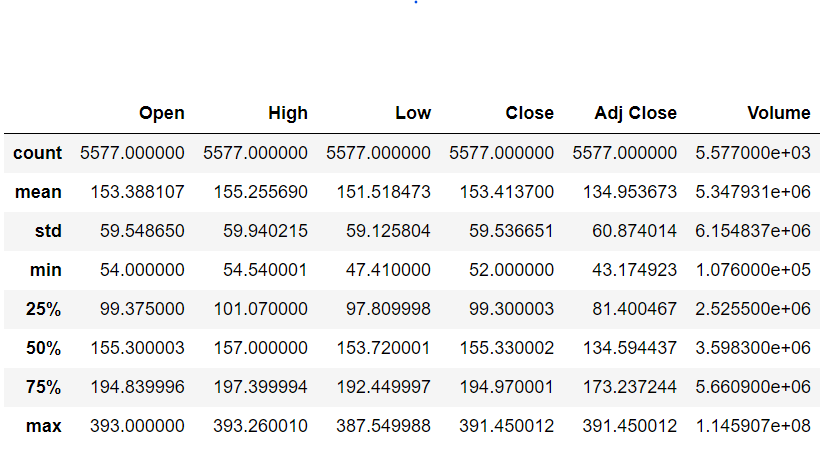
\includegraphics[width=0.9\textwidth]{figures/data.png}
  \caption{Data description without date}\label{data}
\end{figure}

\item \textbf{Brief summary of data exploration}
I 

\item \textbf{Summary of training at least three models} I implemented the game with three different prediction models which are  `RandomForestRegressor, AdaBoostRegressor, and ExtraTreesRegressor'.
    \begin{enumerate}
      \item RandomForestRegressor. It showed the relatively good result. The average step maintaining the pole was 157, with a perfect score of 30 out of 100 trials. (Figure \ref{random_forest})
      \begin{figure}[H]
        \centering
        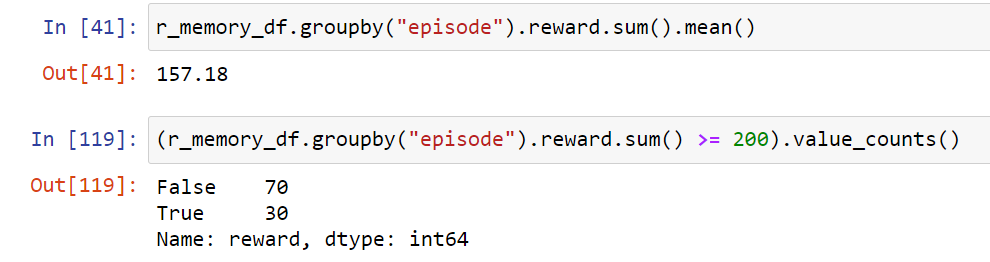
\includegraphics[width=0.9\textwidth]{figures/random_forest.png}
        \caption{RandomForestRegressor}\label{random_forest}
      \end{figure}

      \item AdaBoostRegressor. The result was terrable. Because in the case of AdaBoost it modifies the weights sequencially with the wrongly predicted data set. Since our data set consists of randomly chosen episodes, the AdaBoost model might be inappropriate to train the this data. (Figure \ref{AdaBoost})
      \begin{figure}[H]
        \centering
        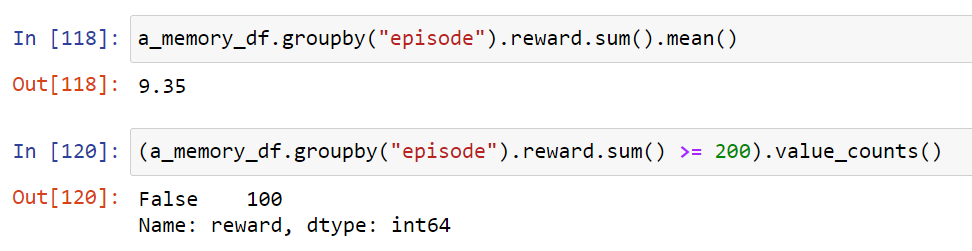
\includegraphics[width=0.9\textwidth]{figures/AdaBoost.png}
        \caption{AdaBoostRegressor}\label{AdaBoost}
      \end{figure}

      \item ExtraTreesRegressor. It showed the relatively good result. The average step maintaining the pole was 138, with a perfect score of 17 out of 100 trials. (Figure \ref{etr})
      \begin{figure}[H]
        \centering
        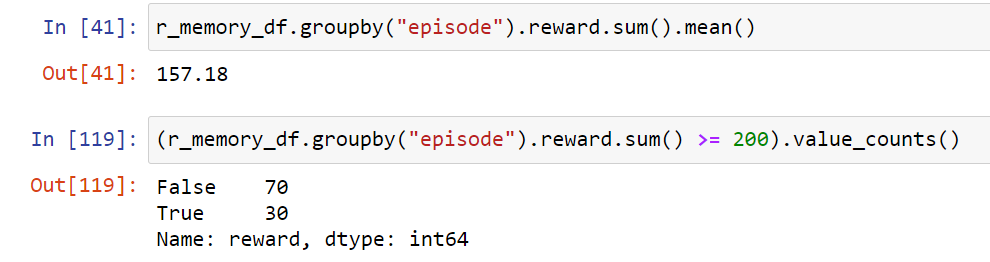
\includegraphics[width=0.9\textwidth]{figures/random_forest.png}
        \caption{ExtraTreesRegressor}\label{etr}
      \end{figure}
    \end{enumerate}

\item \textbf{Explanation of your final model}
Overall, the RandomForestRegressor showed the best performance. I think that this is because we used closely related features to predict the result which are `Cart Position', `Cart Velocity', `Pole Angle', and `Pole Angular velocity'. Thus, the result of RandomForest is better than ExtraTreesRegressor (ETR) because ETR trains the model with randomly chosen features not with all features. In order to increase the performance, I trained the final model (RandomForestRegressor) with more data which have 20000 trials. And the final result shows that the average step maintaining the pole was 157, with a perfect score of 35 out of 100 trials. (Figure \ref{rf2})

\begin{figure}[H]
  \centering
  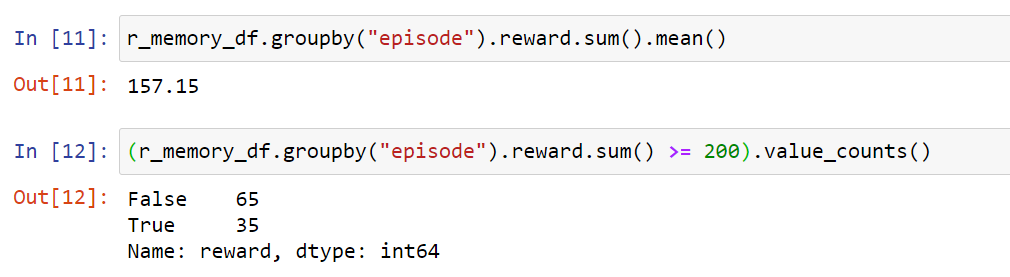
\includegraphics[width=0.9\textwidth]{figures/rf2.png}
  \caption{Final model score}\label{rf2}
\end{figure}

\item \textbf{Summary Key Findings and Insights}
In order to increase the performance, using deep neural network can be another way. Thus I thought about two neural-networks models such as deep neural network, and recurrent neural network for the advanced steps. But in the case of RNN, it seems not to be good to improve the performance because the model is trained based on the episodes which have the same comb\_rewards which is not so related to sequential events. So, I abandoned the RNN. Instead of it, I implemented the Deep Neural Network manually with two hidden layers with (5, 64), (64, 1) dimentions. In the figure \ref{nn}, y-axis shows the error rate. Even though the error rate decreases the total performance was much lower (Average step is 9). I think that this is because when the NN was trained the weights were modified based on individual episode's comb\_rewards which has the same value at the same episode. So, in order to improve the model, the comb\_rewards need to be changed. To be specific, within the same episode, according to the steps increase, the rewards also need to be increased. After I changed the rewards, I was able to check the improved result like represented in the figure \ref{nn_improve}.

\begin{figure}[H]
  \centering
  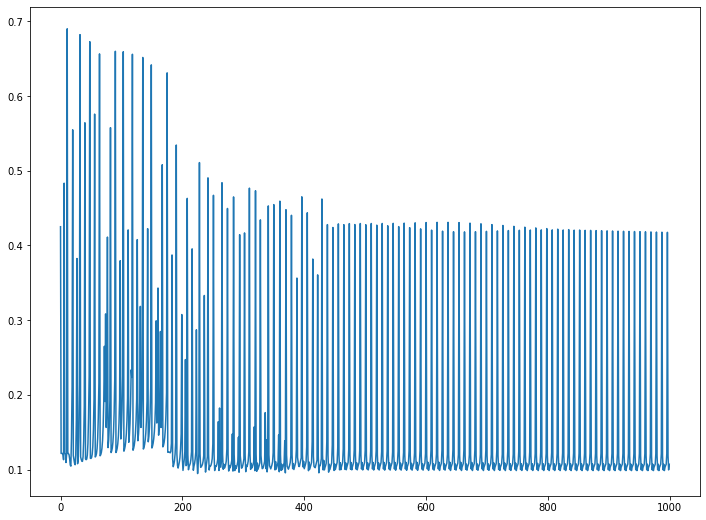
\includegraphics[width=0.9\textwidth]{figures/nn.png}
  \caption{Error of Deep Neural Network model}\label{nn}
\end{figure}

\begin{figure}[H]
  \centering
  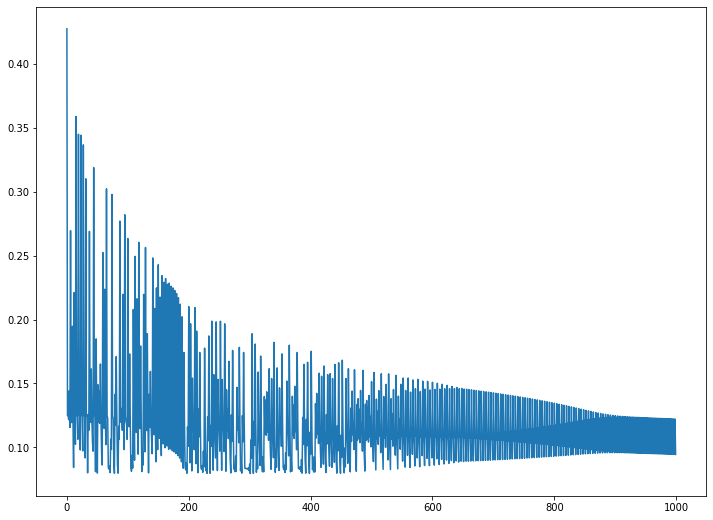
\includegraphics[width=0.9\textwidth]{figures/nn_improve.png}
  \caption{Improved version of DNN}\label{nn_improve}
\end{figure}

\item \textbf{Suggestions for next steps}
When I checked the final result, even though the prediction error was low, the performance was still bed (Average step is 10). I need to find the reason of the poor performance of the Deep Neural Network model.

\end{itemize}

\end {document}